\chapter{Asking Holiday Shoppers How They Got RICH!}

This School of Hard Knocks interview, curated by LazyingArt LLC, is not a lecture in the ordinary blackboard sense, but it does carry a real mathematical structure. The speaker keeps moving from visible wealth to hidden mechanism: from cars and eye-catching income figures to recurring revenue, scalable service, knowledge transfer, capital access, sales, delegation, and execution. Since no validated board or slide images survived from this lecture, the formulas in what follows are cautious reconstructions of the business arithmetic implicit in the transcript rather than transcriptions of visible mathematics.

\section{Hook, Montage, and the Houston Field Site}

The opening montage functions as a preview of variables. Before we are given any explanation, we are given the categories that will govern the rest of the interview: peak annual earnings, exit values, age, age at first millionaire status, and the contrast between wealth now and poverty earlier in life. The host then narrows the scene to Houston's wealthy shopping district and announces the method: we will interrogate wealth one case at a time.

For the sake of clarity, we shall keep the major quantities distinct throughout:
\begin{itemize}
\item \(Y_{\max}\): peak personal earnings in a single year;
\item \(C_{\text{rev}}\): company revenue;
\item \(E\): exit or sale value;
\item \(A\): current age;
\item \(A_{\$}\): age at first millionaire status;
\item \(T\): years spent in an industry or business.
\end{itemize}

This distinction matters immediately. The montage throws out numbers such as \(\$194\) million, \(\$6\) million, and \(\$8\) million, but these are not all the same kind of number. Some refer to company revenue, some to personal yearly earnings, and some to exit value. If we blur them together, the lecture becomes hype. If we separate them, it becomes legible.

The host also frames Houston as an unusually dense environment of wealth and turns the city into a kind of empirical laboratory. The lecture is therefore structured as a field study: each interview is a sample, and each recap is an attempt to extract a law.

\section{Wealth Management and the Arithmetic of Recurring Revenue}

The first full interview supplies the cleanest analytical spine in the lecture. The speaker is in wealth management, has been in finance for \(40\) years, reached millionaire status at age \(36\), and reports a best single year of \(\$6\) million. More important than any one number is the structure of the business he describes. He is not merely chasing isolated transactions; he is building a repeatable service that clients retain over time.

\begin{definition}
A transactional revenue stream is one in which each increment of income requires a fresh deal, a fresh search, or a fresh closing event.
\end{definition}

\begin{definition}
A recurring revenue stream is one in which a client relationship persists across billing periods and continues to pay without restarting the entire acquisition process each time.
\end{definition}

The lecture's basic contrast can be written in deliberately simple form:
\begin{align}
R_{\text{trans}} &\approx N_d f_d, \\
R_{\text{rec}} &\approx N_c\,p\,H\,\rho.
\end{align}
Here \(N_d\) is the number of deals, \(f_d\) is the average value per deal, \(N_c\) is the number of clients, \(p\) is the payment per period, \(H\) is the time horizon, and \(\rho\) is a persistence factor summarizing retention.

The speaker's point is that commercial real estate can make a great deal of money, but each deal sends us back out into the world to find the next deal. A retainer model behaves differently. Once the relationship is established, the revenue stream is carried by continuity rather than repeated search.

\begin{figure}[h]
\centering
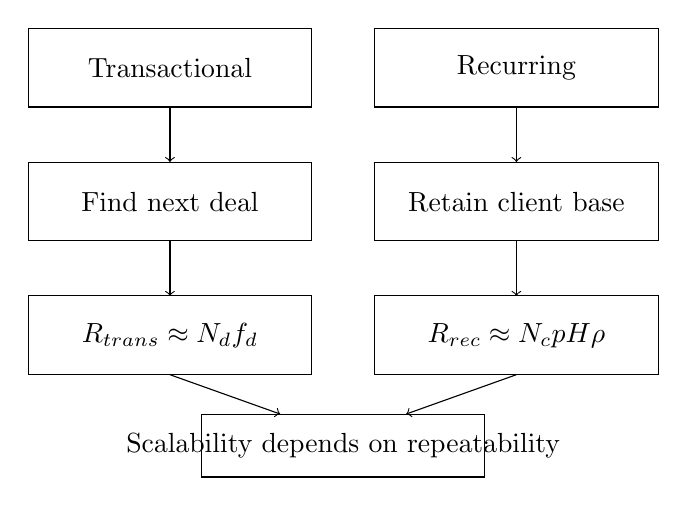
\begin{tikzpicture}[x=1cm,y=1cm]
\draw (0,0) rectangle (3.6,1) node[pos=.5] {Transactional};
\draw (4.4,0) rectangle (8,1) node[pos=.5] {Recurring};

\draw (0,-1.7) rectangle (3.6,-0.7) node[pos=.5] {Find next deal};
\draw (4.4,-1.7) rectangle (8,-0.7) node[pos=.5] {Retain client base};

\draw (0,-3.4) rectangle (3.6,-2.4) node[pos=.5] {\(R_{\text{trans}} \approx N_d f_d\)};
\draw (4.4,-3.4) rectangle (8,-2.4) node[pos=.5] {\(R_{\text{rec}} \approx N_c p H \rho\)};

\draw[->] (1.8,0) -- (1.8,-0.7);
\draw[->] (1.8,-1.7) -- (1.8,-2.4);
\draw[->] (6.2,0) -- (6.2,-0.7);
\draw[->] (6.2,-1.7) -- (6.2,-2.4);

\draw (2.2,-4.7) rectangle (5.8,-3.9) node[pos=.5] {Scalability depends on repeatability};
\draw[->] (1.8,-3.4) -- (3.2,-3.9);
\draw[->] (6.2,-3.4) -- (4.8,-3.9);
\end{tikzpicture}
\caption{Editorial reconstruction of the lecture's central contrast between one-off deal flow and recurring retained revenue.}
\end{figure}

\subsection{Question \& Answer}

Why does recurring, non-transactional revenue scale better than one-off deal flow?

Because the search process is not repeated from zero each time. The lecture never writes this down formally, but its logic is unmistakable. If one unit of service can be standardized, retained, and reused, then time spent building the service does not have to be repaid from scratch with every new customer.

\begin{proposition}
Under the lecture's assumptions, a repeatable retainer model can outgrow a purely transactional model because client count and retention multiply the same underlying process across time.
\end{proposition}

\begin{proof}
The transcript gives a concrete verbal example: one set of transactions can be delivered to about \(100\) different people, and those \(100\) people pay for it. We can formalize that example as follows.
\begin{enumerate}
\item Let the reusable service bundle be fixed.
\item Let \(N_c = 100\) clients purchase that bundle.
\item Let each client pay \(p\) per period.
\item Let the relationship persist over horizon \(H\) with retention factor \(\rho\).
\end{enumerate}
Then the revenue attached to that one service architecture is approximately
\begin{equation}
R_{\text{rec}}^{(100)} \approx 100\,p\,H\,\rho.
\end{equation}
The key feature is not the number \(100\) by itself. The key feature is that the service design cost is not rebuilt from zero for each client. By contrast, in a deal-driven model we remain much closer to
\begin{equation}
R_{\text{trans}} \approx N_d f_d,
\end{equation}
and each increment of \(N_d\) usually requires renewed search, renewed persuasion, and renewed closing effort. Hence, for sufficiently long horizon and sufficiently strong retention, the lecture's preference for recurring revenue is economically intelligible:
\begin{equation}
R_{\text{rec}}(H) > R_{\text{trans}}(H).
\end{equation}
\end{proof}

The host immediately recognizes the pedagogical punchline: schools do not usually teach students to think in this way. The interview is therefore not merely about making money; it is about learning to see the topology of revenue.

\section{From Broke to Trustworthy Practice}

The same wealth-management interview then shifts register. We move from business structure to biography. The speaker reports that he spent the first half of his life broke, came from a divorced household, and experienced a hard upbringing. This is not ornamental detail. It sets up the next question: if the revenue architecture is now clear, how does one become the kind of person to whom that architecture is available?

\subsection{Question \& Answer}

What can someone at rock bottom do right now?

The answer given is not a trick and not a shortcut. It is a sequence of disciplines: pray, learn, stay curious, figure out how things work, and learn to articulate that understanding to others. The lecture's logic here is that knowledge by itself is not enough. Knowledge must become socially legible. People seek out those who are both knowledgeable and trustworthy.

This is where the long-haul theme enters. Earlier the speaker had summarized the best financial advice he received in the language of delayed gratification: many people sacrifice what they want most for what they want now. We may paraphrase the mechanism like this: short-horizon consumption competes with long-horizon compounding. The first victory is therefore not yet scale; it is self-formation. We become, slowly, the sort of operator to whom repeat business can attach.

The interview closes this segment with a character statement rather than a numerical formula: faithfulness to wife, family, and business, followed by the injunction to stay focused and do the right thing. In these notes, that statement should not be treated as a decorative moral flourish. Within the lecture's own structure it is part of the mechanism by which trust is sustained over time.

\section{Cybersecurity, Knowledge, and Time Compression}

The host now recaps the finance lesson in slogan form and pivots sharply into a younger and faster case. A cybersecurity founder reports that he started the company, that it is doing roughly seven figures a month, that he is \(27\) years old, and that he became a millionaire this year. The change in tone is deliberate. The first interview established compounding over decades; this one asks how a much faster trajectory can occur.

The key answer is ignorance. Not ignorance as sin, but ignorance as absence of usable knowledge. The founder then proposes that one can collapse time by seeking the knowledge that has already been allocated to the results one wants.

We can write the lecture's heuristic claim in minimal form as
\begin{equation}
t_{\text{path}} \propto \frac{1}{K_{\text{usable}}},
\end{equation}
where \(t_{\text{path}}\) is the effective time required to reach a result and \(K_{\text{usable}}\) is not abstract information but applied knowledge obtained from those who already know the route.

\subsection{Question \& Answer}

How does knowledge collapse time?

The answer is not that laws of nature are repealed. The answer is that search costs fall. Failed experiments are avoided. We do not have to rediscover every step for ourselves if someone else has already paid that cost and can transmit the pattern.

In the language of the lecture, the derivation is very short:
\begin{enumerate}
\item Decide on a target state.
\item Assume that someone else has already reached it.
\item Acquire the relevant knowledge from that prior operator.
\item Reduce wasted iterations and reduce time lost to blind search.
\end{enumerate}
This is a business-timescale statement, not a physical law, but it is central to the lecture.

The cybersecurity founder then makes a second claim: in the United States, a person who knows how to protect organizations will almost inevitably be paid well. That is a sectoral thesis, not a theorem, but it is part of the lecture's repeated insistence that one should not think only in terms of abstract entrepreneurship. One should ask instead: what problem is economically costly, and what capability is scarce?

The host's recap after this interview is again important. He translates the case into a general statement: what keeps people broke is ignorance, and what reverses that condition is resourcefulness, humility, and purchased knowledge.

\section{Energy, Capital Access, and Timing}

The next interview broadens the frame. The speaker works in energy, oil, and gas, has been in the business for \(35\) years, reports a best single year of \(\$8\) million, and says the company sale was over \(\$740\) million, with contingent language suggesting an even higher upside. Here the lecture moves from knowledge and sales into finance, ownership, and timing.

The most interesting statement in this section is retrospective: if he were to start differently, he would begin in banking rather than in technical geophysics or geology. The reasoning is that technical specialization is excellent, but it often leaves one working for someone else, while finance tells us where the money comes from, who controls it, and how deals are structured.

A compact reconstruction of this point is
\begin{equation}
\mathcal{F}_{\text{technical}} \subsetneq \mathcal{F}_{\text{capital-aware}},
\end{equation}
where \(\mathcal{F}_{\text{technical}}\) is the feasible set available to a purely technical specialist and \(\mathcal{F}_{\text{capital-aware}}\) is the larger set available once one understands financing, ownership, and the flow of capital.

\subsection{Question \& Answer}

Why can capital literacy matter more than pure technical specialization?

Because it changes what actions are available. Technical skill may let us execute a task. Capital literacy lets us choose, finance, structure, and own the task. The lecture does not disparage technical competence; it says rather that technical competence without capital understanding can leave the operator inside a narrower possibility set.

The second decisive move in this section is timing. The founder describes taking risk when Mexico opened up, drilling the first well, and benefiting when that first bet turned out to be large. This is not randomness without structure. It is risk plus positioning plus moment. The lecture's point is that once we understand the capital landscape, the same industry can yield very different outcomes depending on when and how we enter it.

The advice at the end of this interview turns again toward people. Study. Talk to people. Work with good people. Trust compounds not only within client relationships but within partnerships, operating networks, and long careers.

\section{Solar Sales, Immigration, and the Mentor Principle}

The solar-company interview restates several earlier themes but in a different key. The speaker owns a solar company, attributes his growth from six to seven figures to the right people around him, and describes a team structure in which responsibility is distributed rather than hoarded. He also narrates an immigrant path from Honduras, a background of struggle, entry into sales, and later financial success.

What is new here is the sharp defense of commission sales. The speaker is explicit that if one wants to make money in the United States, the decisive move need not be entrepreneurship in the abstract. It may be entry into commission sales. That is a powerful corrective to the lecture's surface imagery. The Lamborghini is not the lesson. The sales skill is.

The lecture also makes a distinction between mentor and guru. Social media may perform wealth without possessing it. Free information is abundant. What remains scarce is the disciplined use of that information and the guidance of someone who has already achieved a concrete result. This theme echoes the cybersecurity section, but now the emphasis is less on sector choice and more on commercial adulthood: work hard, invest in yourself, keep going, and do not confuse visibility with substance.

Just as important is the speaker's account of organizational care. We are told that when we take care of people, those people take care of the business. The lecture is moving, step by step, toward a non-romantic theory of scale: people are not an afterthought to growth; they are one of its primary operating variables.

\section{Lumber, Delegation, and Execution}

The closing interview pushes this people theme into its hardest form. The speaker is in the lumber industry, reports that the company did \(\$194\) million in \(2022\), says he became a millionaire at \(35\), and insists that he is not really in the lumber business but in the people business. The host asks the natural question: what takes a company from eight figures to nine?

The answer is not originality. It is people, delegation, and execution.

We can summarize the lecture's final operating relation as
\begin{equation}
S \approx P\,\Gamma\,X,
\end{equation}
where \(S\) is scale, \(P\) is people quality, \(\Gamma\) is coordination and delegation capacity, and \(X\) is execution quality.

This is not the speaker's notation; it is our compression of his point. The derivation is straightforward:
\begin{enumerate}
\item A founder begins by doing many tasks directly.
\item As the business grows, the founder's attention becomes scarce.
\item If the founder refuses to let go, attention becomes the bottleneck.
\item Hiring strong people increases \(P\).
\item Letting them own parts of the operation increases \(\Gamma\).
\item Focused follow-through increases \(X\).
\item Hence scale grows not from ideation alone but from the organized multiplication of people and execution.
\end{enumerate}

The lecture makes the point in plain language: ideas are cheap, execution is everything. It adds a particularly sharp operational image: the business owner cannot be worried about the price of toilet paper. Once the firm reaches a certain size, local frugality can become a strategic distraction. The founder's work is no longer to touch every object but to shape the system that touches them.

\section{Summary}

The lecture begins with spectacle and ends with structure. Across wealth management, cybersecurity, energy, solar, and lumber, the recurrent laws are remarkably consistent. Wealth is not treated as a mystery but as the result of identifiable mechanisms: delayed gratification, trust, recurring revenue, usable knowledge, capital literacy, sales skill, good people, and execution.

If we compress the whole chapter into a single progression, it is this. First we learn to become trustworthy. Then we learn to build a repeatable revenue process. Then we learn to shorten the path by borrowing tested knowledge. Then we learn to see where capital comes from. Finally, if the business grows large enough, we learn to delegate and execute through other people. That is the interview's real mathematics: not abstract symbolism for its own sake, but the arithmetic of leverage, persistence, and scale.